%------------------------------------------------------------------------------
% Author(s):
% Varaun Ramgoolie
%
% Copyright:
%  Copyright (C) 2020 Brad Bachu, Arjun Mohammed, Varaun Ramgoolie, Nicholas Sammy
%
%  This file is part of Applied-Mathematics-Unit2 and is distributed under the
%  terms of the MIT License. See the LICENSE file for details.
%
%  Description:
%     Year: 2008 May
%     Module: 3
%     Question: 5
%------------------------------------------------------------------------------

\begin{subquestions}
	
\subquestion

%------------------------------------------------------------------------------
% 5 a
%------------------------------------------------------------------------------

\begin{subsubquestions}
	
\subsubquestion

We are given a situation where a collision occurs and two bodies continue moving along the same direction.

\textbf{\textit{Sketch and Translate:}} \\ \\
\begin{figure}[H]
	\begin{center}
		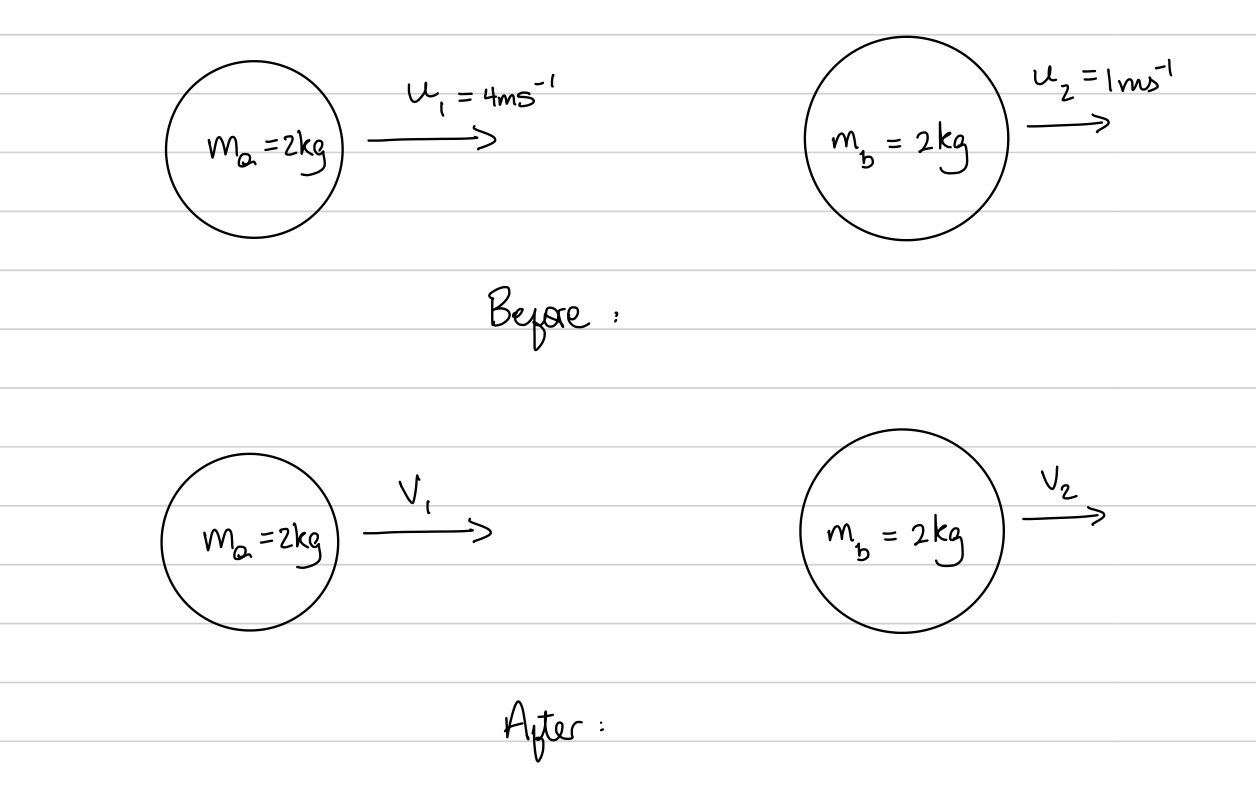
\includegraphics[scale=0.25]{../2007/figures/2008Mq5-1}
		\caption{\label{2008M:q5:Sketch1} Bodies colliding with each other.}
	\end{center}
\end{figure}	
We are asked to find the loss of kinetic energy of the system. As we are given the mass of the bodies, we can use our knowledge of momentum and solve the problem. 



\textbf{\textit{Simplify and Diagram:}} \\ \\
\begin{figure}[H]
	\begin{center}
		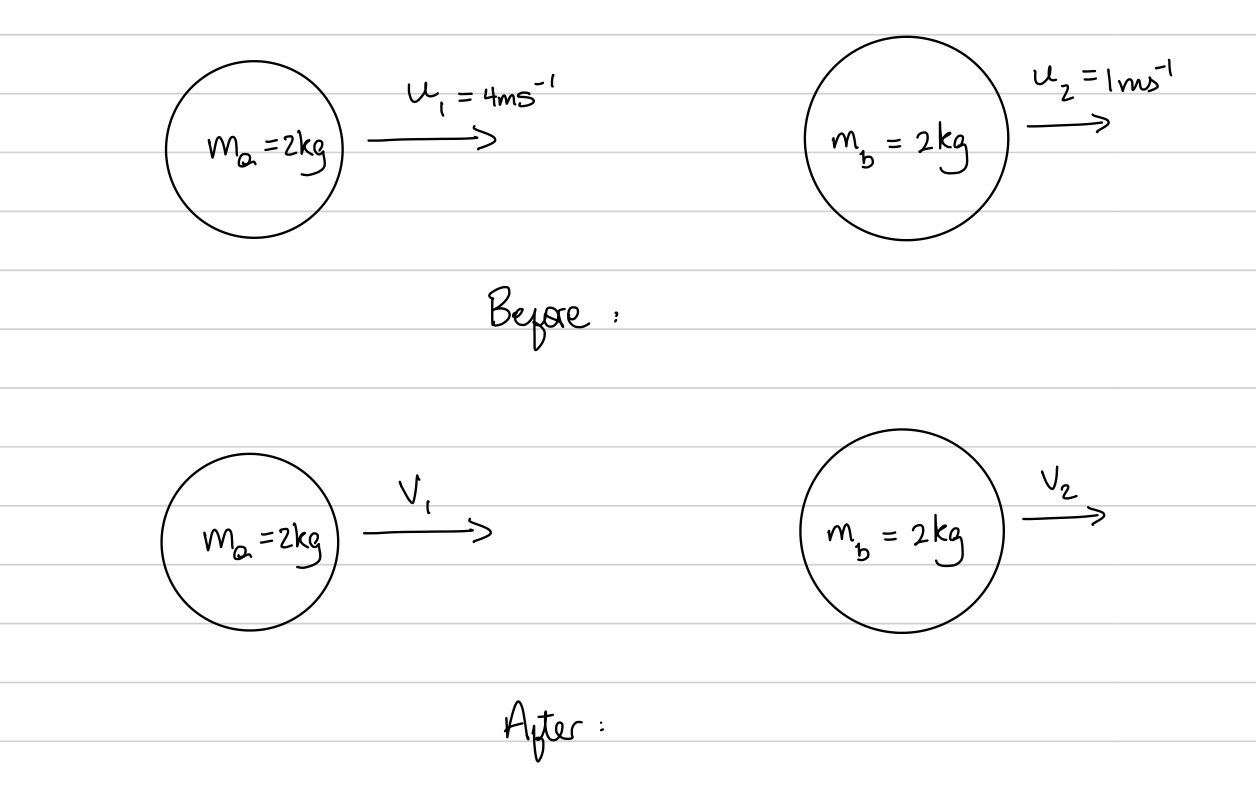
\includegraphics[scale=0.25]{../2007/figures/2008Mq5-1}
		\caption{\label{2008M:q5:Diagram1} Collision overview with velocities and masses.}
	\end{center}
\end{figure}
We will assume that the collision occurs in a closed system (no external forces acting on the system). We will take movement to the right as positive and we will assume that the bodies only move in 1 dimension. We can use the Law of Conservation of Momentum to solve for the final velocities of the spheres and then solve for the change in kinetic energy.




\textbf{\textit{Represent Mathematically:}} \\ \\
From the Law of Conservation of Momentum, we get that,
\begin{align}
	\text{Total Momentum Before collision} & = \text{Total Momentum After collision} \nn \\
	m_Au_A + m_Bu_B & = m_Av_A+m_Bv_B \label{2008M:q5:MomEqn1}\,.
\end{align}

It is also given that,
\begin{equation}
	v_B=2v_A \label{2008M:q5:Speed1} \,.
\end{equation}

Finally, to find the loss of kinetic energy,
\begin{align}
	\Delta \text{Kinetic Energy} & = \text{Initial Kinetic Energy} - \text{Final Kinetic Energy} \nn \\
	                             & = \frac{1}{2}\left(m_Au_A^2+m_Bu_B^2\right) - \frac{1}{2}\left(m_Av_A^2+m_Bv_B^2\right) \label{2008M:q5:KEEqn1} \,.
\end{align}



\textbf{\textit{Solve and Evaluate:}} \\ \\
Firstly, we will substitute $m_A=2$kg, $m_B=2$kg, $u_A=4ms^{-1}$, $u_B=1ms^{-1}$, and $v_B=2v_A$ into \req{2008M:q5:MomEqn1} as,
\begin{align}
	\text{Total Momentum Before collision} & = \text{Total Momentum After collision} \nn \\
	2\times 4 + 2\times 1 & = 2v_A+2v_B \nn \\
	10 & = 2v_A+2(2v_A) \nn \\
	\implies v_A & = \frac{5}{3}ms^{-1} \,.
\end{align}
	
From \req{2008M:q5:Speed1}, we get that,
\begin{align}
	v_B & = 2\times \frac{5}{3} \nn \\
	    & = \frac{10}{3} \,.
\end{align}
	
Substituting our values into \req{2008M:q5:KEEqn1}, we get that,
\begin{align}
	\Delta \text{Kinetic Energy} & = \text{Initial Kinetic Energy} - \text{Final Kinetic Energy} \nn \\
								 & = \frac{1}{2}\left(2\times 16 + 2\times 1\right) - \frac{1}{2}\left(2\times \frac{25}{9}+ 2\times \frac{100}{9}\right) \nn \\
								 & = \frac{28}{9} J \,.
\end{align}
	
%------------------------------------------------------------------------------

\subsubquestion

\textbf{\textit{Simplify and Diagram:}} \\ \\
We can consider \rfig{2008M:q5:Diagram1}. To find the impulse exerted on B by A, we must consider the change in the velocity of sphere B.




\textbf{\textit{Represent Mathematically:}} \\ \\
By definition,
\begin{align}
	\text{Impulse}_{A~on~B} = m_B(v_B-u_B) \label{2008M:q5:Impulse} \,.
\end{align}




\textbf{\textit{Solve and Evaluate:}} \\ \\
Using \req{2008M:q5:Impulse}, we get,
\begin{align}
	\text{Impulse}_{A~on~B} & = 2\times (\frac{10}{3}-1) \nn \\
						    & = \frac{14}{3} kgms^{-1} \,.
\end{align}

\end{subsubquestions}	

%------------------------------------------------------------------------------
% 5 b
%------------------------------------------------------------------------------

\subquestion

\begin{subsubquestions}
	
\subsubquestion

\textbf{\textit{Sketch and Translate:}} \\ \\
We are given the position vector of a particle which is defined by time, $t$. We can consider this as the displacement function, $s(t)$.




\textbf{\textit{Simplify and Diagram:}} \\ \\
By definition, in order to find the velocity of the particle, we must differentiate the displacement function with respect to $t$.




\textbf{\textit{Represent Mathematically:}} \\ \\
The velocity of the particle is given as,
\begin{equation}
	v(t) = \ddd{}{t} s(t) \,.
\end{equation}




\textbf{\textit{Solve and Evaluate:}} \\ \\
The velocity of the particle is,
\begin{align}
	v(t) & = \ddd{}{t} \left(4\sin(t)\ihat + 5\cos(t)\jhat \right) \nn \\
	     & = 4\cos(t) \ihat -5\sin(t) \jhat\,.
\end{align}

The magnitude of the velocity is.
\begin{align}
	|v(t)| = \sqrt{16\cos^2(t)+25\sin^2(t)} \,. 
\end{align}
 
%------------------------------------------------------------------------------

\subsubquestion

\textbf{\textit{Simplify and Diagram:}} \\ \\
By definition, in order to find the acceleration of the particle, we must differentiate the velocity function with respect to $t$.




\textbf{\textit{Represent Mathematically:}} \\ \\
The acceleration of the particle is given as,
\begin{equation}
	a(t) = \ddd{}{t} v(t) \,.
\end{equation}




\textbf{\textit{Solve and Evaluate:}} \\ \\
The acceleration of the particle is,
\begin{align}
	a(t) & = \ddd{}{t} \left(4\cos(t) \ihat -5\sin(t)\jhat \right) \nn \\
	& = -4\sin(t)\ihat - 5\cos(t)\jhat \,.
\end{align}

The magnitude of the acceleration is.
\begin{align}
	|a(t)| = \sqrt{16\sin^2(t)+25\cos^2(t)} \,. 
\end{align}

%------------------------------------------------------------------------------

\subsubquestion

\textbf{\textit{Simplify and Diagram:}} \\ \\
In order to find the momentum of the particle, we will find the product of the particle's mass and velocity.




\textbf{\textit{Represent Mathematically:}} \\ \\
We know that,
\begin{align}
	\text{Momentum} = m \times v(t) \,.
\end{align}




\textbf{\textit{Solve and Evaluate:}} \\ \\
The momentum of the particle is,
\begin{align}
	\text{Momentum} & = 3 \times \left(4\cos(t) \ihat -5\sin(t) \jhat\right) \nn \\
	                & = 12\cos(t) \ihat - 15\sin(t)\jhat \,.
\end{align}

The magnitude of the momentum is,
\begin{align}
	|\text{Momentum}| = \sqrt{144\cos^2(t)+225\sin^2(t)} \,.	
\end{align}

%------------------------------------------------------------------------------

\subsubquestion

\textbf{\textit{Simplify and Diagram:}} \\ \\
In order to find the force on the particle, we will find the product of the particle's mass and acceleration.




\textbf{\textit{Represent Mathematically:}} \\ \\
We know that,
\begin{align}
	F = m \times a(t) \,.
\end{align}




\textbf{\textit{Solve and Evaluate:}} \\ \\
The force on the particle is,
\begin{align}
	F & = 3 \times \left(-4\sin(t)\ihat - 5\cos(t)\jhat\right) \nn \\
	& = -12\sin(t) \ihat - 15\cos(t)\jhat \,.
\end{align}

The magnitude of the force is,
\begin{align}
	|F| = \sqrt{144\sin^2(t)+225\cos^2(t)} \,.	
\end{align}

\end{subsubquestions}

\end{subquestions}